% Insert after the existing Effective Rank discussion, as a separate
% subsection. Preserve the existing oracle-rho results and values.
% Copy fig/rho_proxy_diagnostics.pdf into the manuscript's fig directory.
% Source: results/p1_revision/reused/proxy_summary.json and proxy/*.npz.

\subsection{Effective Rank Estimated from Measurements}
\label{sec:revision-observable-rank}

The true channel is unavailable at the receiver, so the effective rank
used above cannot directly control the estimator. We therefore test a
simple observable proxy: calculate the effective rank from the final
unstructured EM-GS estimate. For user $k$ in trial $i$, define
\begin{equation}
\begin{aligned}
\widehat\rho_{{\rm EM},k,i}
&=\frac{r_{\rm eff}\!\left(\mathcal H(
  \widehat{\mathbf g}_{{\rm EM},k,i})\right)}{r_{\max}},\\
\overline{\widehat\rho}_{{\rm EM},i}
&=\frac{1}{K}\sum_{k=1}^{K}\widehat\rho_{{\rm EM},k,i}.
\end{aligned}
\label{eq:revision-observable-rho}
\end{equation}
We compare this trial-level mean with the corresponding mean from the
true user channels and with the paired HS-GS gain. We use EM-GS estimates
so that the proxy is measured before a Hankel correction changes the
singular values. No true channel or path count is used to form the proxy.

This analysis reuses 10,400 existing Paper~1 trials: 7,200 trials from the
array-size study with $P=30$, and 3,200 trials from the matched $N=32$
complexity study with $P=20$. We repeat only EM-GS using the original
channels, observations, seeds, and update counts. Every reproduced EM-GS
squared error agrees exactly with its stored value in this implementation.
These replays are not additional independent Monte Carlo trials.

Fig.~\ref{fig:revision-observable-rank}(a) shows that the proxy tracks
true effective rank more closely as SNR increases. For $N=32$, the
Spearman correlation rises from $0.202$ at $-5$~dB, with a 95\% interval
of $[0.100,0.297]$, to $0.914$ at $20$~dB, with an interval of
$[0.890,0.931]$. The intervals use 4,000 bootstrap resamples of entire
trials, keeping their user averages and paired errors together.

However, estimation noise raises the proxy substantially. For $N=32$
and SNR $=5$~dB, its mean across trials is $0.577$, whereas the
corresponding true-channel mean is $0.244$. HS-GS still gives a positive
paired-median gain of $2.544$~dB. These are different summaries: the first
two numbers are means of effective rank, while the last is a median of
paired estimation gains. The upward shift warns against applying a cutoff
near $0.5$ to this proxy without calibration. This comparison of averages
does not evaluate a per-trial cutoff.

We also examine the relation between the proxy and HS-GS gain across
path counts. We use the matched $N=32$, $P=20$, RSR $=10$~dB study and
group its random SNRs into fixed 5~dB bands. In the $[-10,-5)$~dB band,
the proxy--gain correlation is $-0.098$, with a 95\% interval of
$[-0.183,-0.012]$. In the $[15,20]$~dB band, it is $-0.797$, with an
interval of $[-0.836,-0.752]$. Negative correlation means that larger
estimated effective rank tends to accompany a smaller structural gain.
The true effective rank and normalized true path count are also shown
as diagnostic references; neither is available to the receiver.

The proxy therefore provides some practical information, especially at
higher SNR. It is not a calibrated replacement for the true effective
rank, and no per-trial rank-selection rule or switching threshold is
validated here. The SNR bands reduce, but do not remove, the influence
of SNR. In this diagnostic we use means over users within each trial;
the original effective-rank curves instead summarize their operating
points by medians over user columns and trials.

\begin{figure*}[!t]
\centering
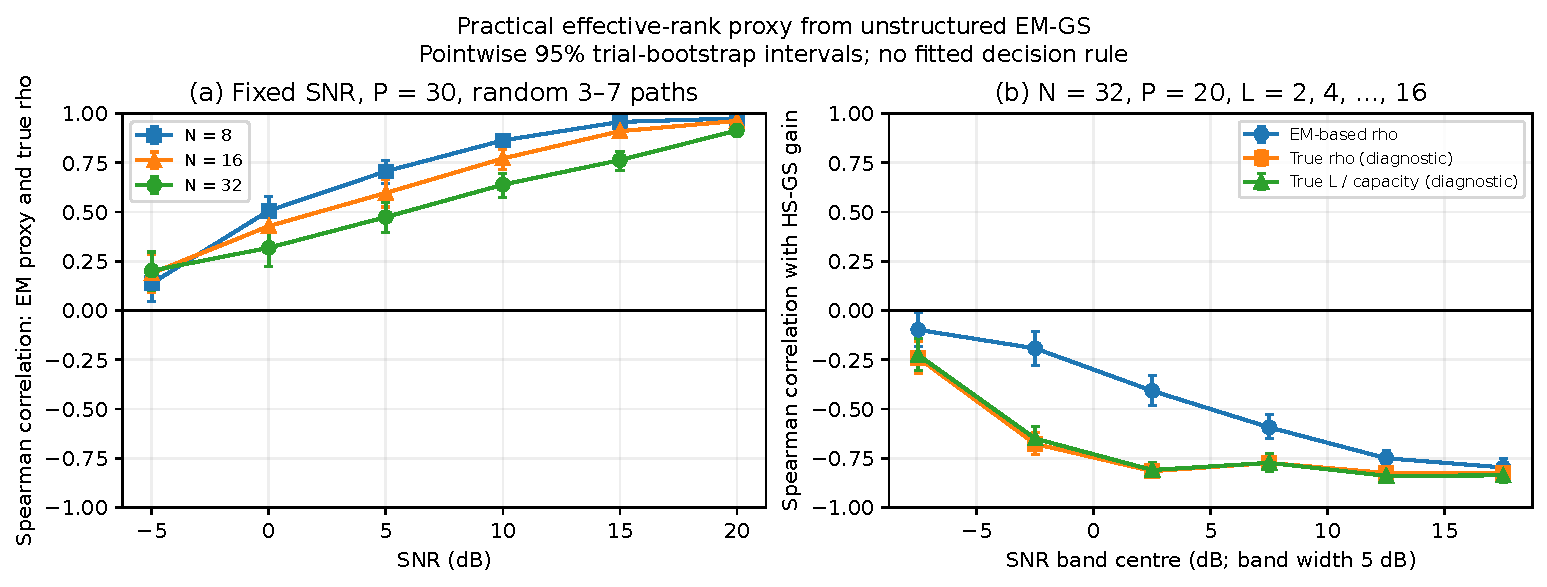
\includegraphics[width=\textwidth]{fig/rho_proxy_diagnostics.pdf}
\caption{Effective rank estimated from unstructured EM-GS.
(a) Correlation between the observable proxy and true effective rank,
using trial-level user means at each fixed SNR.
(b) Correlation with paired HS-GS gain across $L\in\{2,4,\ldots,16\}$
within fixed 5~dB SNR bands. The two true-channel quantities are
evaluation-only references. Error bars are pointwise 95\% intervals
from 4,000 paired trial-bootstrap resamples.}
\label{fig:revision-observable-rank}
\end{figure*}
